\section*{Price Transmission Analysis}

\subsection*{Interpretation}
automate interpretation to a certain extent by learning about circumstances through online data.


\subsection*{Time Series Analysis}
Time series data has a natural temporal relation between different data points.
It is important in the analysis to extract significant temporal statistics out
of data. We will focus on analyze stationarity, autocorrelation, trend, volatility
change, and seasonality of our price datasets in R.

Stationarity of a series guarantees that the mean and variance of the data do not
change over time. This is crucial for a meaningful analysis, since if the data is
not stationary, we can not be sure that anything we derive from the present will
be consistent in the future. We can transform our data into a stationary one by
taking k-th difference to remove the underlying trend, and then apply standard
test procedures such as KPSS test [1] to see if the differenced series is stationary.

Autocorrelation is another important trait in time series data. It suggests the
degree of correlation between different time periods. By plotting correlograms
(autocorrelation plots) of our data, we will be able to identify if the fluctuation
of prices may be due to white noise or other hidden structures.

Seasonality is reasonably expected in our agricultural related time series. Several
methods might help us to detect seasonality, such as common run charts, seasonal
subseries plots, periodograms, and the correolograms we mentioned before.

(trend and volatility change is straightforward and can be concluded once we have the datasets)

[1] Kwiatkowski, D.; Phillips, P. C. B.; Schmidt, P.; Shin, Y. (1992). "Testing the null hypothesis of stationarity against the alternative of a unit root". Journal of Econometrics 54 (1–3): 159–178.


\section*{Prediction Models}

\subsection*{Time Series Forecasting}

\subsubsection*{ARMA Model}
The classical Time series forecasting approach is to use the ARMA (Auto-Regressive
Moving Average) model to predict the target variable as a linear function which
consists of the auto-regressive part (lag variables) and the moving average part
(effects from recent random shocks).

The ARMA(p,q) model: (will refine math representations later)

$Phi(B) * Y_t = Theta(B) * eps_t$

The fitting of the model and the historical
data can be accomplished by maximum likelihood estimation.

\subsubsection*{Regression}
We can also apply ARMA to the linear regression model. It is formulated as such:

$Y = Beta*X + eps,   eps ~ ARMA(p,q)$

Through OLS (Ordinary Leasat Square) or GLS (General Least Square) processes,
we can obtain an optimal Beta.

\subsection*{Multilayer Perceptrons}
taken from M. Seegers course on Pattern Recognition and ML

\subsection*{Recurrent Neural Networks (RNN)}
source: scholarpedia
A recurrent neural network (RNN) is a neural network in with feedback connections, enabling signals to be fed back from a layer $l$ in the network to a previous layer. %The key feature is that the weight matrix for each layer $l$ in the network contains input weights from \emph{all} other neurons in the network and not just the neurons from the previous layer. 

\subsubsection*{Simple Recurrent Networks}
The simplest form of an RNN consists of an input, an output and one hidden layer as depicted in fig.[]. 

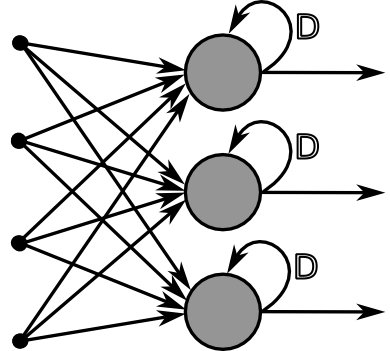
\includegraphics[width=.7\textwidth]{./img/simple_rnn.png}
[source: wikipedia]

\subsubsection*{General description of a discrete time RNN}
A discrete time RNN is a graph with $K$ input units $\vec{u}$, $N$ internal network units $\vec{x}$ and $L$ output units $\vec{y}$. The activation (per layer) vectors at point n in time are denoted by $\vec{u}(n) = (u_1(n),...,u_n(n))$, $\vec{x}(n) = (x_1(n),...,x_n(n))$, $\vec{y}(n) = (y_1(n),...,y_n(n))$. Edges between the units in these sets are represented by weights $\omega_{ij}\neq0$ which are gathered in adjacency matrices. There are four types of matrices:\par
\begin{itemize}
	\item $\vec{W}^{in}_{N\times K}$ contains inputs weigths for an internal unit in each row respectively 
	\item $\vec{W}_{N\times N}$ contains the internal weights. This matrix is usually sparse with densities $5\%-20\%$
	\item $\vec{W}^{out}_{L\times (K+N+L)}$ contains the weights for edges, which can stem from the input, the internal units and the outputs themselves, leading to the output units.
	\item $\vec{W}^{back}_{N\times L}$ contain weights for the edges that project back from the output units to the $N$ internal units
\end{itemize}

In a \emph{fully recurrent network} every unit receives input from all other units neurons and therefore input units can have direct impact on output units. Output units can further be interconnected.\par

\paragraph{Evaluation}
The calculation of the new state of the internal neurons in time-step $n+1$ is called evalution. 
\[
\vec{x}(n+1)=\vec{f}(\vec{W}^{in}\vec{u}(n+1)+\vec{W}\vec{x}(n)+\vec{W}^{back}\vec{y}(n))
\]
where $f=(f_1,...,f_N)$
\paragraph{Exploitation}
The output activations are then computed from the internal state of the network in the exploitation step.
\[
\vec{y}(n+1)=f^{out}(\vec{W}^{out}(\vec{u}(n+1),\vec{x}(n+1),\vec{y}(n)))
\]
where $f^{out}=(f^{out}_1,...,f^{out}_L)$ are the output activation functions and the matrix of output weights is multiplied by the concatenation of input, internal and previous output activation vectors.\par

%A \emph{Hopfield network} is an RNN all connections of which are symmetric and which requires stationary inputs. 
RNNs can in theory approximate any dynamical system with chosen precision, however training them is very difficult in practice. 

\subsection*{Echo State Networks}
Echo State Networks (ESN) are a type of discrete time RNNs for which training is straightforward with linear regression methods.  The temporal inputs to the network are transformed to a high-dimensional \emph{echo state}, described by the neurons of a sparsely connected \emph{random} hidden layer which is also called a reservoir. The output weights are the only weights in the network that can change and are trained in a way to match the desired output. ESNs and the related liquid state machines (LSMs) form the field of \emph{reservoir computing}.

\subsubsection{Echo State Property}
The intuitive meaning of the \emph{echo state property} (ESP) is that the internal state is \textbf{uniquely} determined by the history of the input signal and the teacher forced output, given that the network has been running long enough. Teacher forcing essentially means that the output $\vec{y}(n-1)$ is forced to be equal to the next time series value $\vec{u}(n)$ and thus to the next input.
\begin{frm-def}
For every left infinite sequence $(\vec{u}(n),\vec{y}(n-1)),n=\dots,-2,-1,0$ and all state sequences $\vec{x}(n),\vec{x'}(n)$ which are generated according to
\begin{align*}	
	\vec{x}(n+1)=\vec{f}(\vec{W}^{in}\vec{u}(n+1)+\vec{W}\vec{x}(n)+\vec{W}^{back}\vec{y}(n))\\
	\vec{x'}(n+1)=\vec{f}(\vec{W}^{in}\vec{u}(n+1)+\vec{W}\vec{x'}(n)+\vec{W}^{back}\vec{y}(n))
\end{align*}
it holds true that $\vec{x}(n)=\vec{x'}(n)$ for all $n \leq 0$.
\end{frm-def}
The echo state propery is ensured through the matrix of internal weights $W$

\begin{frm-thm}
Define $\sigma_{max}$ as largest singular value of $\vec{W}$, $\lambda_{max}$ as largest absolute eigenvalue of $\vec{W}$.
\begin{enumerate}
\item If $\sigma_{max} < 1$ then the ESP holds for the network
\item If $\|\lambda_{max}\| > 1$ then the network has no echo states for any input/output interval which contains the zero input/output tuple (0,0)
\end{enumerate}
\end{frm-thm}

\subsubsection*{Training the ESN}
"The state of the ESN is therefore a function of the finite history of the inputs presented to the network. Now, in order to predict the output from the states of the oscillators the only thing that has to be learned is how to couple the outputs to the oscillators, i.e. the hidden to output connections:"
http://stackoverflow.com/questions/21940860/echo-state-network-learning-mackey-glass-function-but-how

Hyperparameters: dimensionality of W, spectral radius $\alpha$
\paragraph*{Teacher forcing}

\paragraph*{Ridge Regression}

\paragraph*{Initial state determination}
The network is run for a first set of inputs and the results are then discarded. If the spectral radius is close to unity, implying slow forgetting of the starting state, the initial set has to be a substantial part of the training dataset.

"Likewise, when the trained network is used to predict a sequence, a long initial run of the sequence must be fed into the network before the actual prediction can start. This is a nuisance because such long initial transients are in principle unneccessary"

"By contrast, a recurrent neural network such as our echo state network, but also such as the networks used in [5] need long initial runs to “tune in” to the to-be-predicted sequence. [5] tackle this problem by training a second, auxiliary “initiator” network."
EchoStatesTechRep.pdf, p.32

\begin{comment}
\subsubsection*{Finding the right topology for the specific prediction problem}

\subsubsection*{Converge}
conceive network that converges fast to speed up training\par
"Known supervised training techniques for RNNS comprise Back Propagation Through Time (BPTT), Real Time Recurrent Learn- ing (RTRL) or Extended Kalman Filtering (EKF) all of which have some major drawbacks."
{\em Application of BPTT to RNNs requires stacking identical copies of the network thus unfolding the cyclic paths in the synaptic connections. Unlike back-propagation used in feed-forward nets, BPTT is not guaranteed to con- verge to a local error minimum, computational cost is O(TN2) per time step where N is the number of nodes, T the number of epochs. In contrast RTRL needs O((N + L)4) (L denotes number of output units), which makes this algorithm only applicable for small nets. The algorithm complexity of EKF is O(LN2). EKF is mathematically very elaborate and only a few experts have trained predefined dynamical system behaviors successfully}\par


\subsubsection*{Avoiding overfitting}

\cite{jaeger_echo_state_RNN}
The third section explains how echo state networks can be trained in a
supervised way. The natural approach here is to adapt only the weights
of network-to-output connections. Essentially, this trains readout functions
which transform the echo state into the desired output signal. Technically,
this amounts to a linear regression task.
\end{comment}


